\section{Lenguaje de programación}

\paragraph{}
Una de las decisiones más importante que consideraba a la hora de desarrolla el proyecto, era la elección de un lenguaje de 
programación adecuado y que cumpliera todas las expectativas necesarias. En un principio se pensó en utilizar C++ por varias 
razones:

\begin{enumerate}
    \item Lenguaje que hemos visto y aprendido a lo largo de toda la carrera, y con más profundidad en la asignatura de 
    Programación Orientada a Objetos. Por lo que ya se tenía una soltura y conocimientos
    previos que no se tenían con ningún otro lenguaje.
    
    \item Lenguaje compilado por lo que su velocidad y eficiencia es mucho mayor que la de otros lenguajes. Aspectos 
    muy a tener en cuenta a la hora de desarrollar un videojuego.
\end{enumerate}

\paragraph{}
Aún así, vamos a desarrollar un juego en 2D por lo que quizás las exigencias tanto de eficiencia como velocidad no son tan altas,
como las de un juego en 3D. También debía tener en cuenta que era la ocasión perfecta para poder aprender un nuevo lenguaje de 
programación, ya que no hay forma mejor de aprender uno que desarrollando un proyecto.

\paragraph{}
Tras evaluar varias posibilidades y todos sus virtudes y defectos, me decanté por elegir como lenguaje de programación para el 
desarrollo del proyecto, el lenguaje \emph{Python}. A continuación se verán las distintas ventajas y desventajas de este lenguaje 
comparadas con C++:

\begin{enumerate}
    \item Multiplataforma al igual que C++ por lo que no tendremos problemas para portar el proyecto a otras plataformas.
    
    \item Lenguaje interpretado que a diferencia de C++, que es compilado, puede ser más lento que este.
    
    \item Sintaxis muy limpia y que favorece a un código mucho más legible.
    
    \item A la par de una sintaxis limpia, una gran facilidad para aprenderlo, también posee una documentación inmensa.
    
    \item Conjunto de bibliotecas estándar muy amplia y muy bien documentadas.
    
    \item Lenguaje multiparadigma, soporta orientación a objetos, programación imperativa y programación funcional.
\end{enumerate}

\begin{figure}[H]
  \label{logo_python}
  \begin{center}
    
\includegraphics[scale=0.4]{imagenes/logo_python.png}
  \end{center}
  \caption{Herramientas utilizadas: Logo de python}
\end{figure}

\paragraph{}
Así que finalmente se decidió usar \emph{Python} como lenguaje principal para el desarrollo de \emph{Zycars} y cabe destacar que se han obtenido
unos resultado muy satisfactorios y ha cumplido todas las expectativas esperadas.

\section{Biblioteca gráfica}

\paragraph{}
Tras la decisión final del lenguaje de programación que se usaría a lo largo de todo el desarrollo del proyecto, la siguiente
decisión de gran importancia que se debía tomar, era la elección de la
biblioteca gráfica que usaríamos en \emph{Zycars}.

\paragraph{}
En este caso se tuvo clara la elección desde el momento en el que se decidió usar \emph{Python} como lenguaje principal, me decanté
por la biblioteca gráfica \emph{Pygame}. Dicha biblioteca es un wrapper de la biblioteca \emph{SDL}, de C/C++, para \emph{Python}, por
lo que tiene todas las virtudes de dicha biblioteca:

\begin{enumerate}
    \item Biblioteca multiplataforma compatible oficialmente con los sistemas Microsoft Windows, GNU/Linux, Mac OS y QNX.
    
    \item Programada en C, por lo que tiene un gran rendimiento.
    
    \item Muy completa, ya que permiten la manipulación tanto de imágenes 2D, como gestión de sonido y música, y también gestión
    de la entrada estándar del sistema. Todos los elementos necesario para el desarrollo de videojuegos.
    
    \item También se usó durante el desarrollo de la asignatura de Diseño de Videojuegos, por lo que se conocen todas sus 
    características muy bien.
\end{enumerate}

\begin{figure}[H]
  \label{logo_pygame}
  \begin{center}
    
\includegraphics[scale=0.6]{imagenes/logo_pygame.png}
  \end{center}
  \caption{Herramientas utilizadas: Logo de pygame}
\end{figure}

\paragraph{}
A parte de todas las virtudes que tiene heredadas de la \emph{SDL}, \emph{Pygame} tiene un nivel de abstracción más alto, por lo que
el uso de esta se hace mucho más sencillo y llevadero, sin necesidad de realizar una abstracción propia, como se haría con la 
\emph{SDL} al usar programación orientada a objetos.

\section{Analizador de código: Pylint}

\paragraph{}
Se creyó necesario que el código que se implementara siguiera un estándar
uniforme y que estuviera exento de cualquier tipo de 
errores o signos de mala calidad. Para ello se usó la herramienta Pylint.

\paragraph{}
Pylint es una herramienta que analiza el código \emph{Python} en busca de errores y señales de mala calidad. Es una herramienta 
de python que comprueba si un módulo cumple con un estándar de codificación.

\paragraph{}
Nos ofrece multitud de funcionalidades, como la comprobación de la longitud de las líneas de código, comprobación si los nombres de 
las variables están bien formadas de acuerdo a su estándar de codificación, o comprobar si las interfaces declaradas son realmente 
implementadas.

\paragraph{}
La gran ventaja de pylint es que es altamente configurable y personalizable, y es muy fácil escribir un pequeño plugin para 
añadir una característica personal.

\section{Sistema de control de versiones}

\paragraph{}
Todo el código y recursos de \emph{Zycars} está alojado en el sistema que proporciona Google Code, que consiste en un entorno completo
usando el sistema de control de versiones \emph{subversion}.

\paragraph{}
Nos permite llevar todas las versiones y visualizar todos los cambios que se han producido durante todo el desarrollo del proyecto,
entre los distintos archivos del mismo, así como poder volver a versiones anteriores en caso de necesidad y cualquier operación
que permita cualquier sistema de control de versiones.

\paragraph{}
Se evaluaron otros sistema de control de versiones como pueden ser GIT o mercurial \footnote{Google Code también permite la gestión
de proyecto mediante Mercurial}, pero finalmente me decanté por subversión, ya
que en el proyecto yo era el único desarrollador y 
quizás, los otros dos sistema están pensados para proyectos con un número de más altos
desarrolladores.

\section{Documentación del código}

\paragraph{}
Para la documentación del código me decanté por usar \emph{Doxygen}, esta permite la documentación sencilla y legible de todo el 
código, generando la documentación en varios formatos como puede ser \emph{HTML} o \emph{PDF}.

\paragraph{}
Para python existe la herramienta \emph{Doxypy}, que nos permite usar la convención de comentarios de \emph{Python} y adaptarlos a
\emph{Doxygen}, por lo que nos ahorra trabajo y sigue la normativa de código \emph{Python}.

\paragraph{}
También comentar que dicha herramienta se usó en proyectos anteriores con resultados muy satisfactorios.

\section{Redacción de la memoria.}

\paragraph{}
Para la completa realización de la memoria se ha usado \LaTeX. Es un sistema de composición de textos, orientado 
especialmente a la creación de libros, documentos científicos y técnicos que contengan fórmulas matemáticas.

\begin{figure}[H]
  \label{logo_latex}
  \begin{center}
    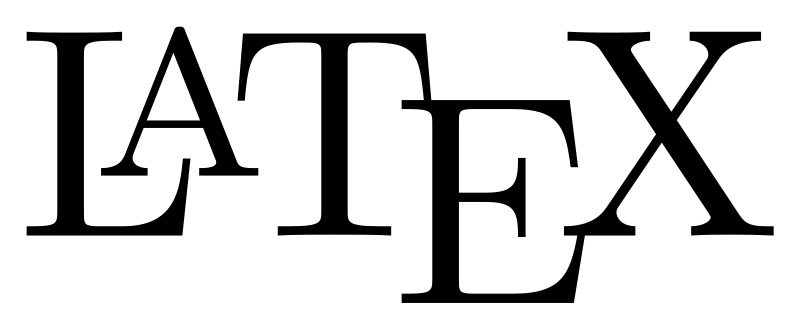
\includegraphics[scale=0.25]{imagenes/logo_latex.png}
  \end{center}
  \caption{Herramientas utilizadas: Logo de \LaTeX}
\end{figure}

\paragraph{}
\LaTeX es un sistema de composición de textos que está formado mayoritariamente por órdenes (macros) construidas a partir de 
comandos de TeX. \LaTeX es una herramienta práctica y útil pues, a su facilidad de uso, se une toda la potencia de TeX.

\section{Realización de diagramas: Dia}

\paragraph{}
Para la realización de todos los diagramas necesarios que aparecen a lo largo de toda la memoria se ha usado el creador de 
diagramas Dia.

\paragraph{}
Dia es un programa de creación de diagramas en GNU/Linux, MacOS X, Unix y Windows, bajo la 
licencia GPL. Puede ser utilizado para dibujar diferentes tipos de diagramas. Actualmente cuenta con herramientas para dibujar 
diagramas entidad relación, diagramas UML, diagramas de flujo, diagramas de red, y muchos otros diagramas.

\section{Programa de edición de escenarios: Tiled}

\paragraph{}
Como se comenta en el capítulo referente a la implementación del proyecto, se
dejó claro que los circuito y niveles que aparecen
en el juego estarán formados por tiles. Dicho formato se podría usar ficheros de texto plano indicando la posición de 
los tiles, pero se eligió una opción muchísimo más cómoda y con resultado muchos mejores.

\begin{figure}[H]
  \label{tiled_logo}
  \begin{center}
    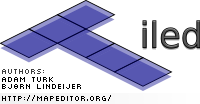
\includegraphics[scale=1]{imagenes/tiled_logo.png}
  \end{center}
  \caption{Herramientas utilizadas: Logo de Tiled}
\end{figure}

\paragraph{}
Para ello se eligió el programa de edición de mapas \emph{Tiled}, el mismo es
un editor de mapas de tiles de propósito general.
Está hecho para ser fácil de usar, lo suficientemente flexible para trabajar con distintos motores de juegos, como RPG, carreras... 
\emph{Tiled} es software libre y escrito en C++, usando la librerías gráficas QT. Las principales características son las siguientes

\begin{itemize}
    \item Generación de XML con la información de todo el mapa.
    
    \item Soporta mapas ortogonales e isométricos.
    
    \item Objetos personalizados pueden ser colocados con precisión de píxeles.
    
    \item Agregar propiedades personalizadas a los tiles, capas u objetos del mapa.
    
    \item Redimensionar tamaño de mapas sin problemas.
    
    \item Soporta entrada y salida de plugins para abrir y guardar archivos en formatos personalizados.
\end{itemize}

\begin{figure}[H]
  \label{captura_tiled}
  \begin{center}
    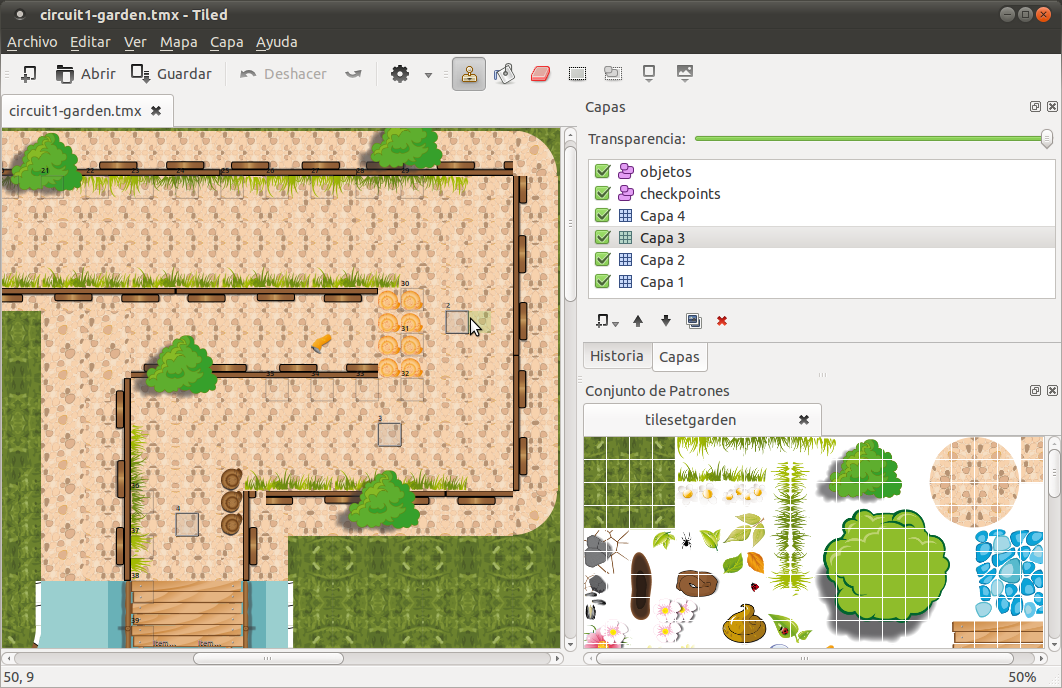
\includegraphics[scale=0.35]{imagenes/captura_tiled.png}
  \end{center}
  \caption{Herramientas utilizadas: Captura del editor de mapas Tiled}
\end{figure}
